\subsection{Descriptions}

\FloatBarrier

\begin{figure}[h!]
	\centering
	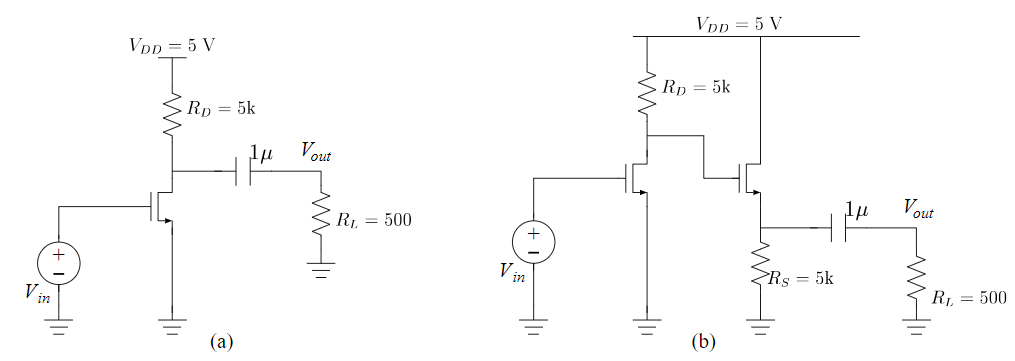
\includegraphics[scale=0.60]{./images/circuit_3.PNG}
	\caption{Amplifiers with Loads and Decoupling Capacitors}
	\label{fig:circuit_3}
\end{figure}

\FloatBarrier

The common-source amplifier is constructed with a $1$\si{\micro\farad} decoupling capacitor and $500$\si{\ohm} load at the output.
The decoupling capacitor ensures that the output has a DC bias of $0$\si{\volt} since any DC voltage simply charges the capacitor and does not make it to the resistor.
The gain is determined at different frequencies.
Again, the gain degrades at higher frequencies due to the parasitic capacitances of the MOSFET acting as a low-pass filter, which cuts down on the signal's amplitude.
A common-drain amplifier is then connected to the output of the common-source amplifier.

\subsection{Calculations}

Because of the attached load, only $\frac{R_{L}}{r_{out} + R_{L}}V_{in}$ ends up appearing at the output, where $r_{out}$ is the amplifier's output resistance.
Since $R_{L}$ is comaparable in magnitude to $r_{out}$, the voltage division effect causes the gain to be much lower than an ideal open circuit gain, measured in part $2$.

% Gain for CSA
\FloatBarrier

\begin{table}[h!]
	\centering
	\caption{Common-Source Amplifier with Decoupling Capacitor and Load Gain}
	\label{tab:gain_part3}
	\csvautotabular{./tables/gain_part3.csv}
\end{table}

\FloatBarrier

The common-drain amplifier's output resistance is given by $r_{out,CDA} = R_{S} || r_{o} || \frac{1}{g_{m}}$.
Assuming $r_{o}$ is very large, $r_{out,CDA} \approx R_{S} || \frac{1}{g_{m}}$.
The common-source amplifier's output resistance is given by $r_{out,CSA} = R_{D} || r_{o}$.
Making the same assumption about $r_{o}$, $r_{out,CSA} \approx R_{D}$. \\

In this specific case, $R_{S} = R_{D} = R$.
Expanding $r_{out,CDA}$, the equation can be rewritten as:

\begin{equation}
	\label{eq:r_out_cda}
	r_{out,CDA} = \frac{R}{1+g_{m}R}
\end{equation}

Likewise, $r_{out,CSA}$ can be written as:

\begin{equation}
	\label{eq:r_out_csa}
	r_{out,CSA} = R
\end{equation}

Assume $R > 0$\si{\ohm} and $g_{m} > 0 \frac{mA}{V}$.
$g_{m}R > 0$ must then be true.
This further implies that $1 + g_{m}R > 1$ and that $\frac{1}{1 + g_{m}R} < 1$.
Because $R > 0$\si{\ohm}, $\frac{R}{1 + g_{m}R} < R$.
Invoking equations (\ref{eq:r_out_cda}) and (\ref{eq:r_out_csa}), $r_{out,CDA} < r_{out,CSA}$. \\

Therefore, in this configuration, the cascaded amplifier should have a lower output resistance since the output is presented with $r_{out,CDA}$ and not $r_{out,CSA}$.
As a result, for the same load, the gain should be higher since $R_{L}$ is now relatively larger in the voltage divider.

\FloatBarrier

\begin{table}[h!]
	\centering
	\caption{Two-Stage Amplifier with Decoupling Capacitor and Load Gain}
	\label{tab:gain_part3_cascade}
	\csvautotabular{./tables/gain_part3_cascade.csv}
\end{table}

\FloatBarrier

\subsection{Analysis}

\FloatBarrier

\begin{figure}[h!]
	\centering
	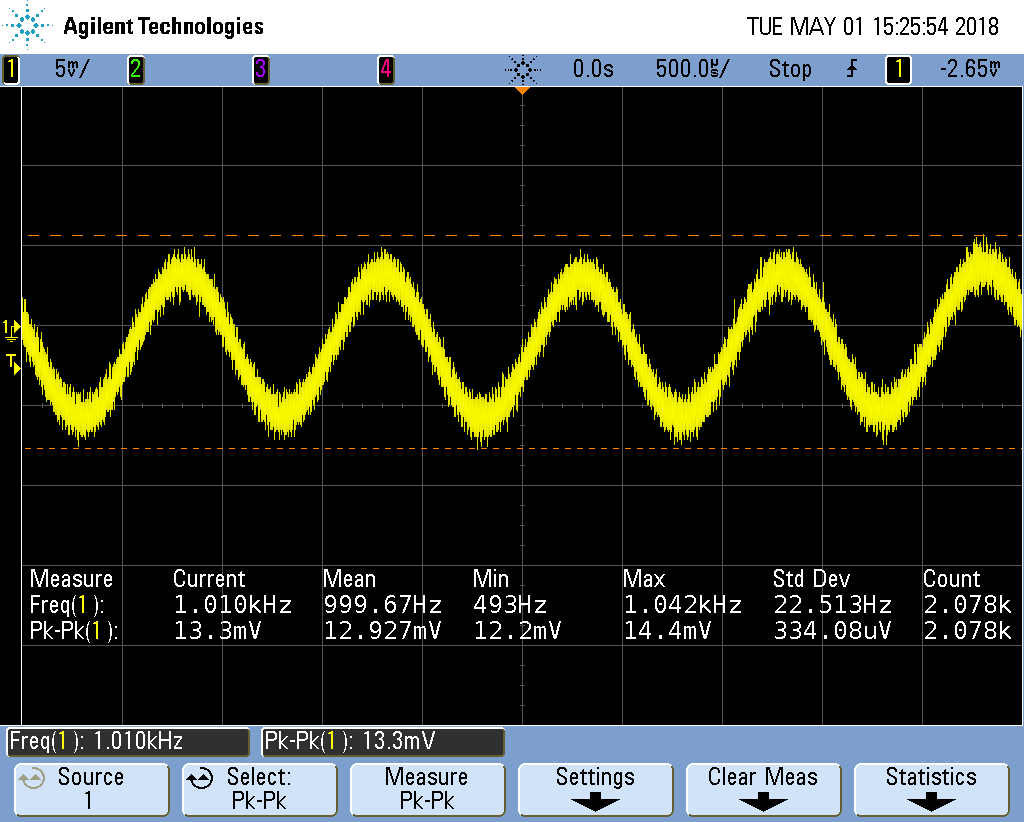
\includegraphics[scale=0.45]{./images/SCOPE_13.PNG}
	\caption{Common-Source Amplifier with Load and Decoupling Capacitors, $1$\si{\kilo\hertz} Input}
	\label{fig:SCOPE_13}
\end{figure}

\FloatBarrier

\begin{figure}[h!]
	\centering
	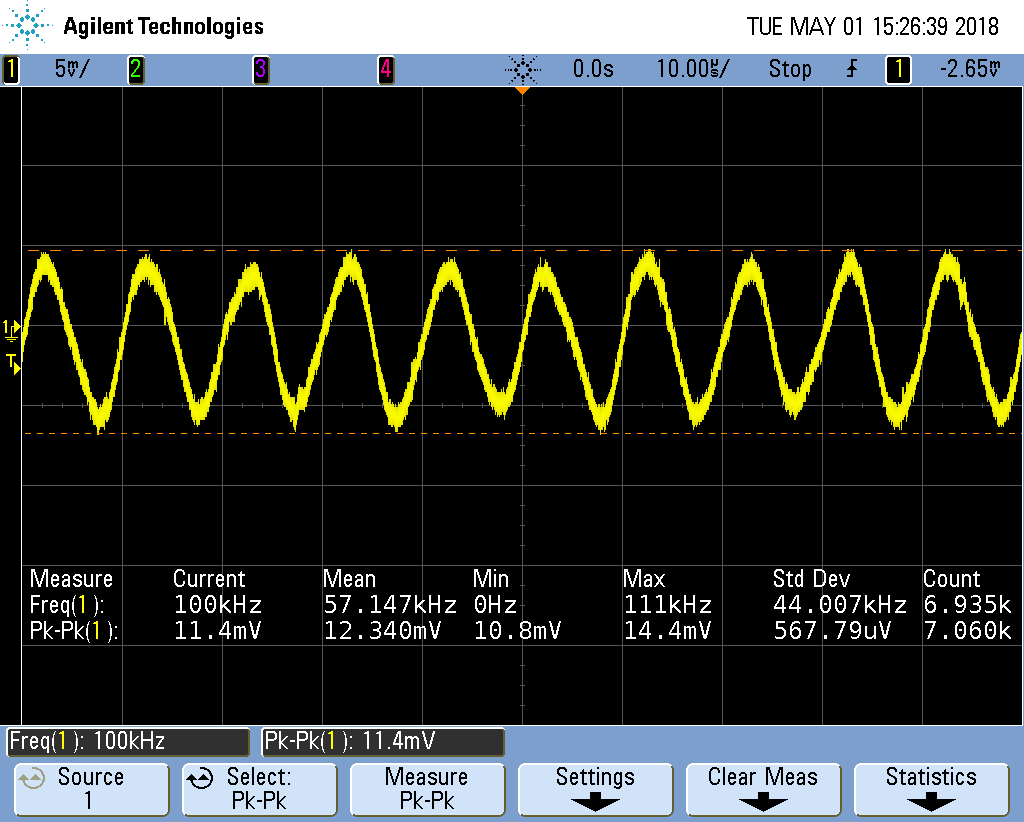
\includegraphics[scale=0.45]{./images/SCOPE_14.PNG}
	\caption{Common-Source Amplifier with Load and Decoupling Capacitors, $100$\si{\kilo\hertz} Input}
	\label{fig:SCOPE_14}
\end{figure}

\FloatBarrier

\begin{figure}[h!]
	\centering
	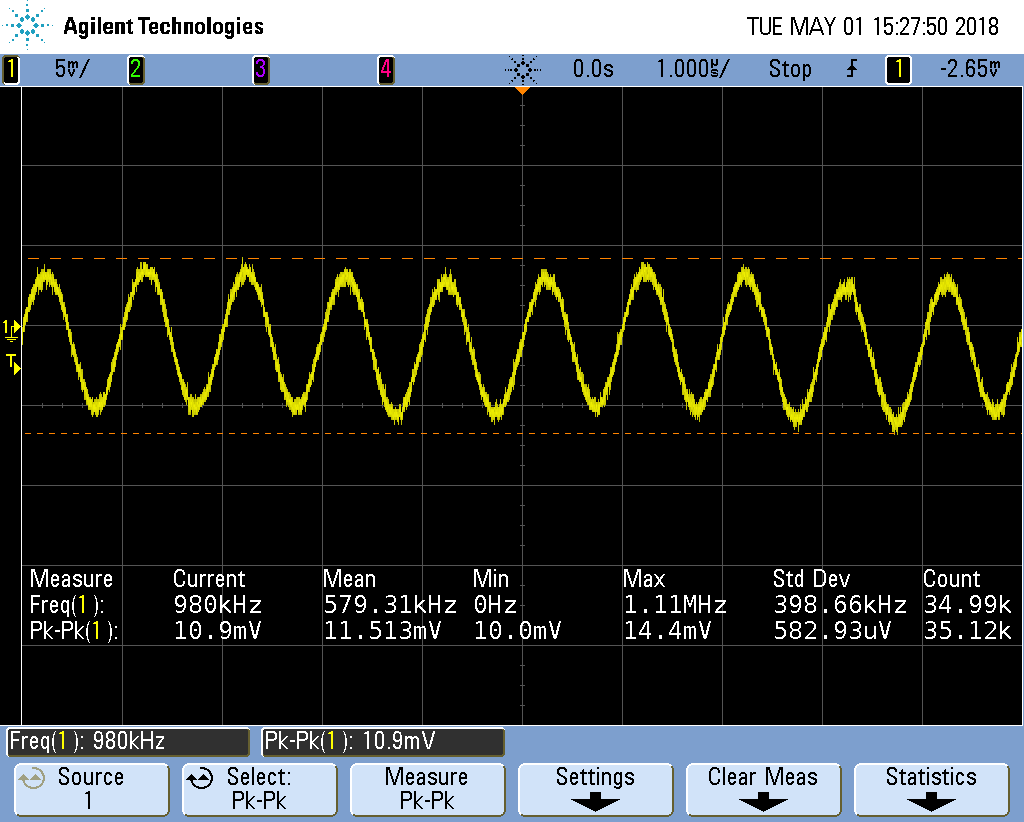
\includegraphics[scale=0.45]{./images/SCOPE_15.PNG}
	\caption{Common-Source Amplifier with Load and Decoupling Capacitors, $1$\si{\mega\hertz} Input}
	\label{fig:SCOPE_15}
\end{figure}

\FloatBarrier

\begin{figure}[h!]
	\centering
	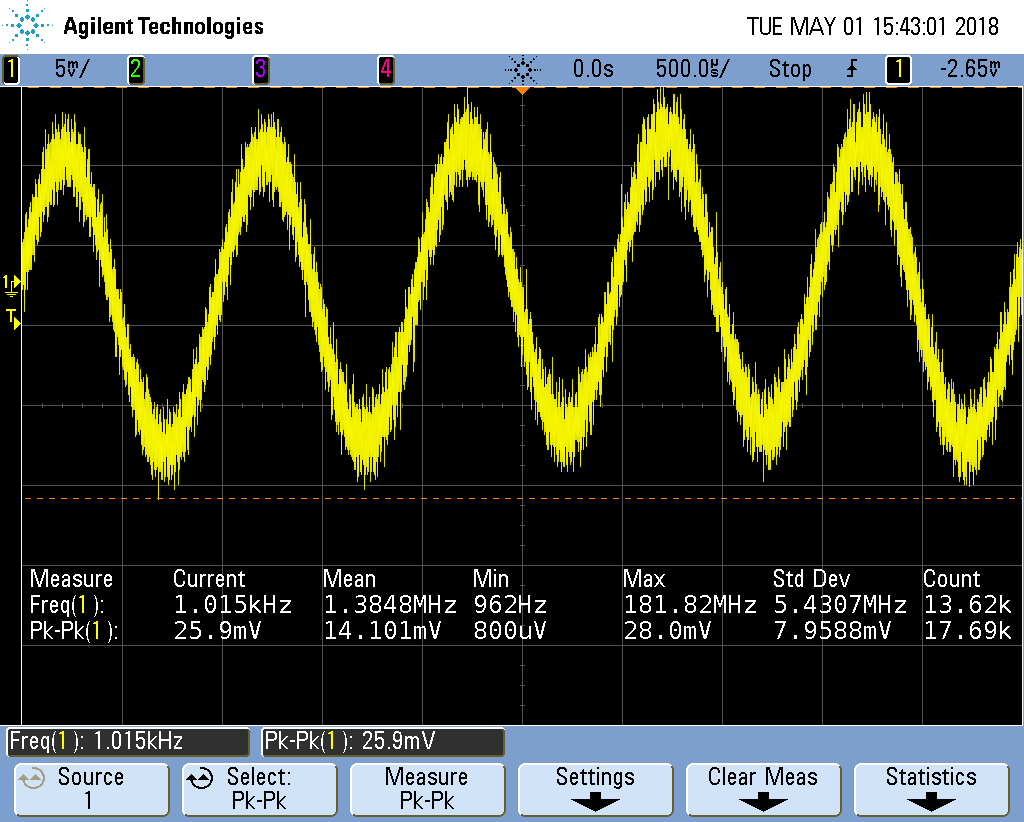
\includegraphics[scale=0.45]{./images/SCOPE_18.PNG}
	\caption{Two-Stage Amplifier with Load and Decoupling Capacitors, $1$\si{\kilo\hertz}}
	\label{fig:SCOPE_18}
\end{figure}

\FloatBarrier

\begin{figure}[h!]
	\centering
	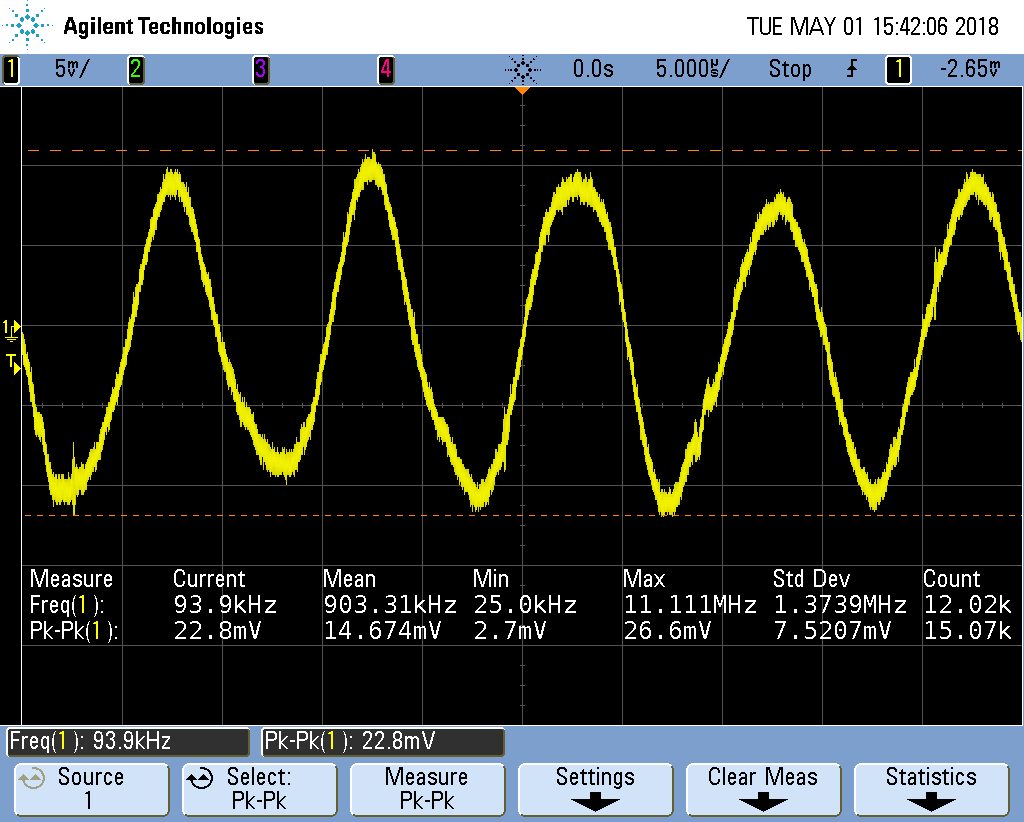
\includegraphics[scale=0.45]{./images/SCOPE_17.PNG}
	\caption{Two-Stage Amplifier with Load and Decoupling Capacitors, $100$\si{\kilo\hertz}}
	\label{fig:SCOPE_17}
\end{figure}

\FloatBarrier

\begin{figure}[h!]
	\centering
	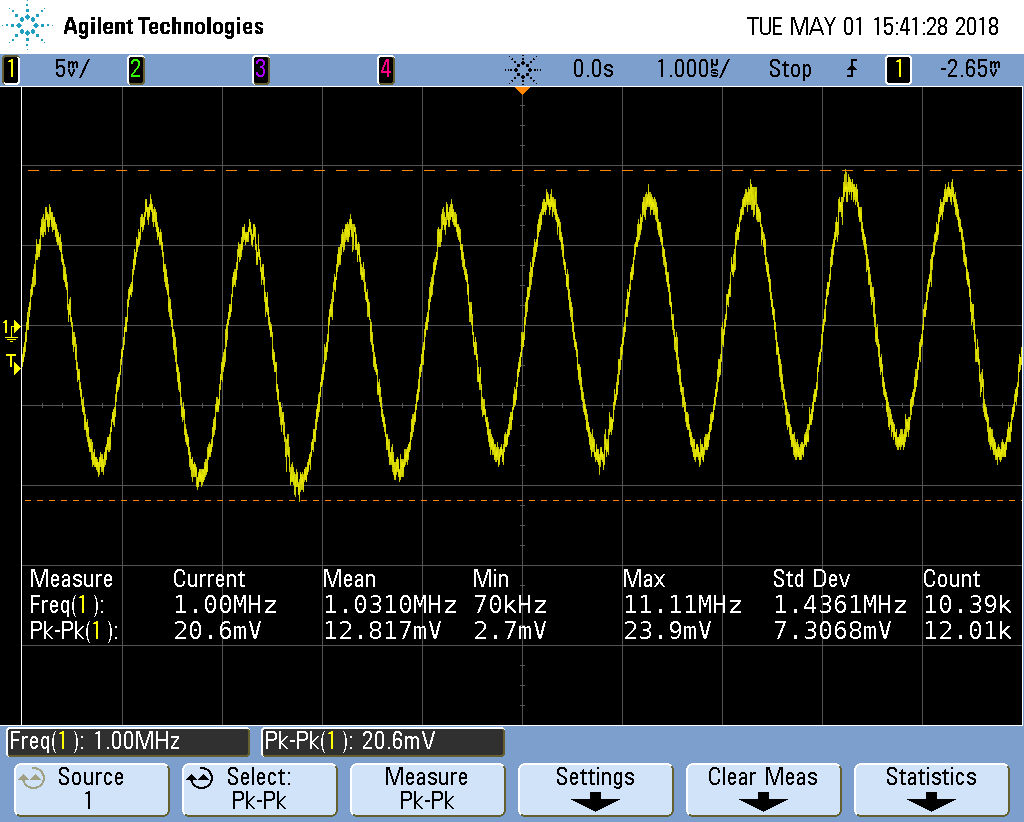
\includegraphics[scale=0.45]{./images/SCOPE_16.PNG}
	\caption{Two-Stage Amplifier with Load and Decoupling Capacitors, $1$\si{\mega\hertz}}
	\label{fig:SCOPE_16}
\end{figure}

\FloatBarrier

The amplifier's gain increases as a result of attaching the common-drain amplifier at the output.
This claim is corroborated by the data at various frequencies.
